\section{Architecture}
\label{sec:architecture}

This section provides detailed technical specifications for both \supra{} and \zennano{} models, including their architectural components, optimization strategies, and implementation details.

\subsection{Base Architecture: Qwen3-4B}

Both models build upon the \qwen{} 4B architecture, which incorporates several state-of-the-art techniques for efficient language modeling:

\subsubsection{Transformer Architecture}
The base architecture follows the standard transformer decoder structure with the following specifications:

\begin{table}[H]
\centering
\begin{tabular}{lr}
\toprule
Parameter & Value \\
\midrule
Hidden Size ($d_{model}$) & 2,560 \\
Intermediate Size ($d_{ff}$) & 9,728 \\
Number of Layers ($L$) & 36 \\
Number of Attention Heads ($h$) & 32 \\
Number of Key-Value Heads & 8 \\
Head Dimension ($d_k$) & 128 \\
Vocabulary Size & 151,936 \\
Maximum Position Embeddings & 32,768 \\
Extended Position Embeddings & 131,072 (YaRN) \\
Total Parameters & 4,022,458,880 (4.02B) \\
Non-Embedding Parameters & 3.63B \\
\bottomrule
\end{tabular}
\caption{Qwen3-4B base model architectural parameters (verified specifications)}
\label{tab:base-architecture}
\end{table}

\subsubsection{Advanced Components}

\textbf{Rotary Position Embeddings (RoPE)}: We employ RoPE for position encoding, which provides several advantages over traditional absolute position embeddings:

\begin{align}
\mathbf{q}_m &= \mathbf{R}_m \mathbf{W}_q \mathbf{x}_m \\
\mathbf{k}_n &= \mathbf{R}_n \mathbf{W}_k \mathbf{x}_n
\end{align}

where $\mathbf{R}_m$ and $\mathbf{R}_n$ are rotation matrices encoding positions $m$ and $n$, respectively.

\textbf{SwiGLU Activation}: The feed-forward networks use SwiGLU activation instead of standard ReLU:

\begin{align}
\text{SwiGLU}(\mathbf{x}) &= \text{Swish}(\mathbf{x} \mathbf{W}_1) \odot (\mathbf{x} \mathbf{W}_2) \\
\text{Swish}(\mathbf{x}) &= \mathbf{x} \cdot \sigma(\mathbf{x})
\end{align}

\textbf{RMSNorm}: Layer normalization is replaced with Root Mean Square Layer Normalization for improved training stability:

\begin{align}
\text{RMSNorm}(\mathbf{x}) = \frac{\mathbf{x}}{\sqrt{\frac{1}{d} \sum_{i=1}^{d} x_i^2}} \odot \mathbf{g}
\end{align}

where $\mathbf{g}$ is a learnable scaling parameter.

\subsection{Supra Nexus o1: Thinking Model Architecture}

\supra{} is specifically designed for transparent reasoning tasks with explicit thinking processes.

\subsubsection{Thinking Token Integration}

The model learns to structure its output using special thinking tokens:

\begin{lstlisting}[caption=Thinking token structure,label=lst:thinking-tokens]
<thinking>
[Internal reasoning process]
- Problem analysis
- Step-by-step solution
- Verification
</thinking>

[Final answer presentation]
\end{lstlisting}

The thinking tokens serve as structural delimiters that separate internal reasoning from the final response, enabling:
\begin{itemize}
    \item Complete transparency in problem-solving approach
    \item Error detection in reasoning steps
    \item Educational value through demonstrated methodology
    \item Improved reliability through explicit verification
\end{itemize}

\subsubsection{Training Objective Modifications}

For \supra{}, we modify the standard language modeling objective to encourage structured thinking:

\begin{align}
\mathcal{L} = \mathcal{L}_{\text{thinking}} + \lambda \mathcal{L}_{\text{answer}}
\end{align}

where:
\begin{itemize}
    \item $\mathcal{L}_{\text{thinking}}$ is the loss on thinking content
    \item $\mathcal{L}_{\text{answer}}$ is the loss on final answer
    \item $\lambda$ balances the two components (set to 0.7)
\end{itemize}

\subsection{Zen Nano: Instruct Model Architecture}

\zennano{} is optimized for direct instruction following with efficiency as a primary concern.

\subsubsection{Identity Integration}

\zennano{} incorporates identity information directly into its training data, ensuring consistent self-representation:

\begin{figure}[H]
\centering
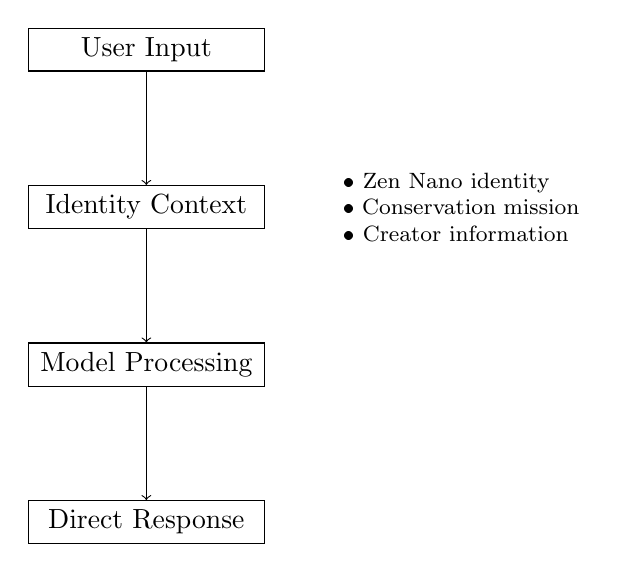
\begin{tikzpicture}[node distance=2cm, auto]
    \node[draw, rectangle, minimum width=3cm] (input) {User Input};
    \node[draw, rectangle, minimum width=3cm, below of=input] (identity) {Identity Context};
    \node[draw, rectangle, minimum width=3cm, below of=identity] (processing) {Model Processing};
    \node[draw, rectangle, minimum width=3cm, below of=processing] (output) {Direct Response};
    
    \draw[->] (input) -- (identity);
    \draw[->] (identity) -- (processing);
    \draw[->] (processing) -- (output);
    
    \node[right of=identity, node distance=4cm] {\begin{minipage}{3cm}
        \footnotesize
        • Zen Nano identity\\
        • Conservation mission\\
        • Creator information
    \end{minipage}};
\end{tikzpicture}
\caption{Zen Nano processing pipeline with identity integration}
\label{fig:zen-nano-pipeline}
\end{figure}

\subsubsection{Optimization for Efficiency}

\zennano{} incorporates several optimizations for efficient inference:

\begin{itemize}
    \item \textbf{Reduced Context Length}: Optimized for shorter interactions
    \item \textbf{Direct Response Training}: Minimizes reasoning overhead
    \item \textbf{Conservation-Focused Knowledge}: Domain-specific optimization
    \item \textbf{Compact Representations}: Efficient knowledge encoding
\end{itemize}

\subsection{LoRA Integration}

Both models employ Low-Rank Adaptation for parameter-efficient fine-tuning:

\subsubsection{LoRA Mathematics}

For a linear layer with weight matrix $\mathbf{W} \in \mathbb{R}^{d \times k}$, LoRA introduces trainable matrices $\mathbf{A} \in \mathbb{R}^{r \times k}$ and $\mathbf{B} \in \mathbb{R}^{d \times r}$ where $r \ll \min(d,k)$:

\begin{align}
h &= \mathbf{W}_0 x + \Delta \mathbf{W} x \\
\Delta \mathbf{W} &= \mathbf{B}\mathbf{A} \\
h &= \mathbf{W}_0 x + \frac{\alpha}{r} \mathbf{B}\mathbf{A} x
\end{align}

where $\alpha$ is a scaling hyperparameter.

\subsubsection{Target Module Selection}

We apply LoRA to the following transformer components:

\begin{table}[H]
\centering
\begin{tabular}{lcc}
\toprule
Module & Parameters & Rank \\
\midrule
Query Projection ($\mathbf{W}_q$) & 2560×4096 & 8 \\
Key Projection ($\mathbf{W}_k$) & 2560×1024 & 8 \\
Value Projection ($\mathbf{W}_v$) & 2560×1024 & 8 \\
Output Projection ($\mathbf{W}_o$) & 4096×2560 & 8 \\
\bottomrule
\end{tabular}
\caption{LoRA target modules and configurations (GQA-adjusted dimensions)}
\label{tab:lora-modules}
\end{table}

This configuration results in only 0.67\% of parameters being trainable during fine-tuning, significantly reducing computational requirements while maintaining performance.

\subsection{MLX Framework Optimization}

Our implementation leverages Apple's MLX framework for optimized performance on Apple Silicon:

\subsubsection{Memory Optimization}

MLX's unified memory architecture allows for efficient memory utilization:

\begin{itemize}
    \item \textbf{Unified Memory Access}: Direct GPU-CPU memory sharing
    \item \textbf{Dynamic Memory Allocation}: Automatic memory management
    \item \textbf{Memory Mapping}: Large model loading optimization
    \item \textbf{Gradient Checkpointing}: Memory-efficient training
\end{itemize}

\subsubsection{Quantization Strategies}

We employ 8-bit quantization for deployment:

\begin{align}
\mathbf{W}_{int8} = \text{round}\left(\frac{\mathbf{W}_{fp16}}{\text{scale}}\right)
\end{align}

where the scale factor is computed per-channel for optimal precision preservation.

\subsubsection{Kernel Optimization}

MLX provides hardware-specific kernel implementations:

\begin{itemize}
    \item \textbf{Matrix Multiplication}: Optimized GEMM kernels
    \item \textbf{Attention Computation}: Fused attention operations
    \item \textbf{Activation Functions}: Vectorized implementations
    \item \textbf{Normalization}: Hardware-accelerated norm computations
\end{itemize}

\subsection{Performance Characteristics}

\begin{table}[H]
\centering
\begin{tabular}{lcc}
\toprule
Metric & \supra{} & \zennano{} \\
\midrule
Inference Speed (tokens/sec) & 45 & 52 \\
Memory Usage (GB) & 8.4 & 8.1 \\
FP16 Model Size (GB) & 8.04 & 8.04 \\
INT8 Quantized Size (GB) & 4.02 & 4.02 \\
INT4 Quantized Size (GB) & 2.01 & 2.01 \\
Training Time (hours) & 2.5 & 1.8 \\
Parameters (Total) & 4.02B & 4.02B \\
Parameters (Trainable LoRA) & 205K & 205K \\
\bottomrule
\end{tabular}
\caption{Performance characteristics on Apple M2 MacBook Pro (corrected specifications)}
\label{tab:performance}
\end{table}

The next section details our training procedures and optimization strategies.